% Intro
This section describes the architectures of the legacy and new systems that will be run and measured in the experimental part of this thesis. The section is divided into four sections and each schema presented shows the protocol step by step.

\subsection{Legacy system - Writing}
\label{subsec:legacy_sys_writing}

Figure \ref{fig:featurestore_writing}~\footnote{For enhanced visualization, refer Figure~\ref{fig:appx_featurestore_writing}} shows the legacy Hopsworks Feature Store write process from the client onto the Offline Feature Store. The process is mainly split into two synchronous parts: upload and materialization. In the upload step, the Pandas data frame given as input is converted into rows and sent one row at a time to Kafka. Then, when the upload is finished the client is notified. Asynchronously, a Spark job has been running in the cluster since the Hopsworks cluster was started, which is the Hudi Delta Streamer. This job periodically retrieves messages from Kafka, and then once it retrieves a full table it writes it in a column-oriented format to Apache Hudi, which sits on top of a \gls{HopsFS} system. Once the materialization is completed the Python client is also notified of completion.

As in the pipeline, the upload and the materialization are two different parts of the process that do not act synchronously. During the experimental part of the thesis, to be able to measure the latency of the whole process without having to account for the Hudi Delta Streamer data retrieval period, the materialize function was called, which allows the system to perform the materialization on call instead of waiting for the period. This enabled the experiments to retrieve accurate data on the total latency of the process.

\begin{figure}
    \begin{center}
      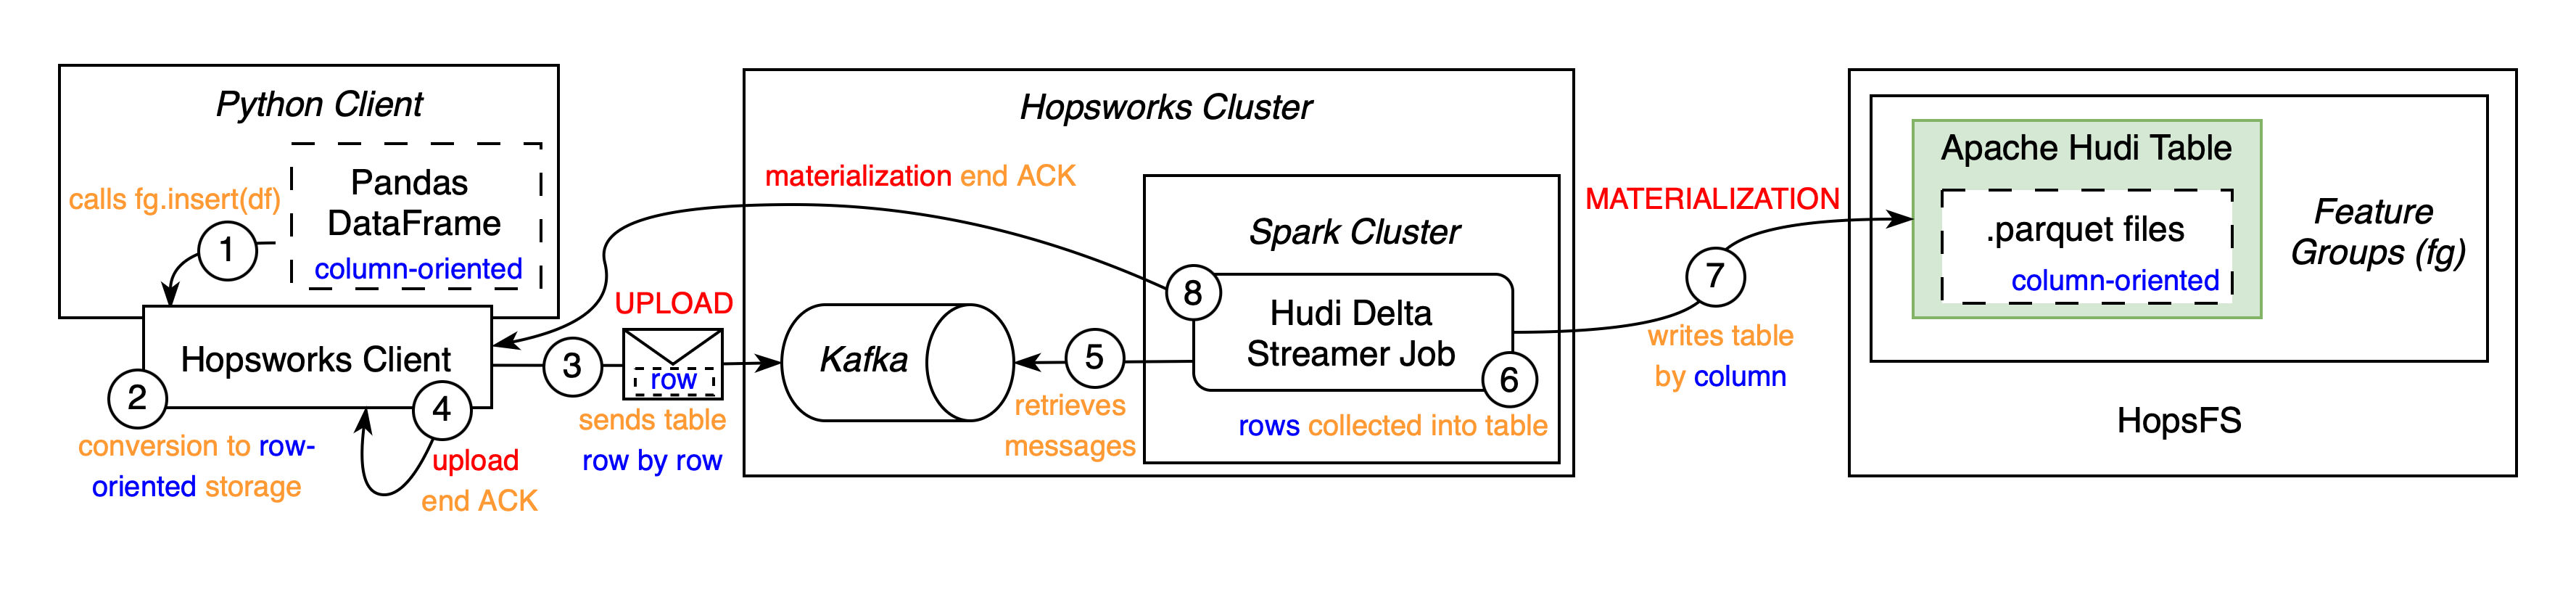
\includegraphics[width=\textwidth]{figures/2-background/FeatureStore-writing.png}
    \end{center}
    \caption[Legacy system - Write process]{Legacy system writing a Pandas data frame from a Python client to the Hopsworks offline Feature Store. Each step is represented with a number. In blue it is outlined the table format conversion, i.e. from columns to rows and then from row to columns. Steps from one to four represent the upload process, while the materialization process in complete at step eight. Diagram realized based on one-to-one interviews with Hopsworks AB employees developing the Hopsworks Feature Store.}
    \label{fig:featurestore_writing}
\end{figure}

\subsection{Legacy system - Reading}
\label{subsec:legacy_sys_reading}

Figure \ref{fig:featurestore_reading}~\footnote{For enhanced visualization, refer Figure~\ref{fig:appx_featurestore_reading}} shows the legacy Hopsworks Feature Store read process from the client onto the Offline Feature Store. The process, differently from the writing process, is not Spark-based and it is using a Spark alternative: a combination of an Arrow Flight server and a DuckDB instance. This avoids the serialization and deserialization into row-based tables for sending the data, keeping the unified standard Arrow Table, which is a column-oriented format.

\begin{figure}
    \begin{center}
      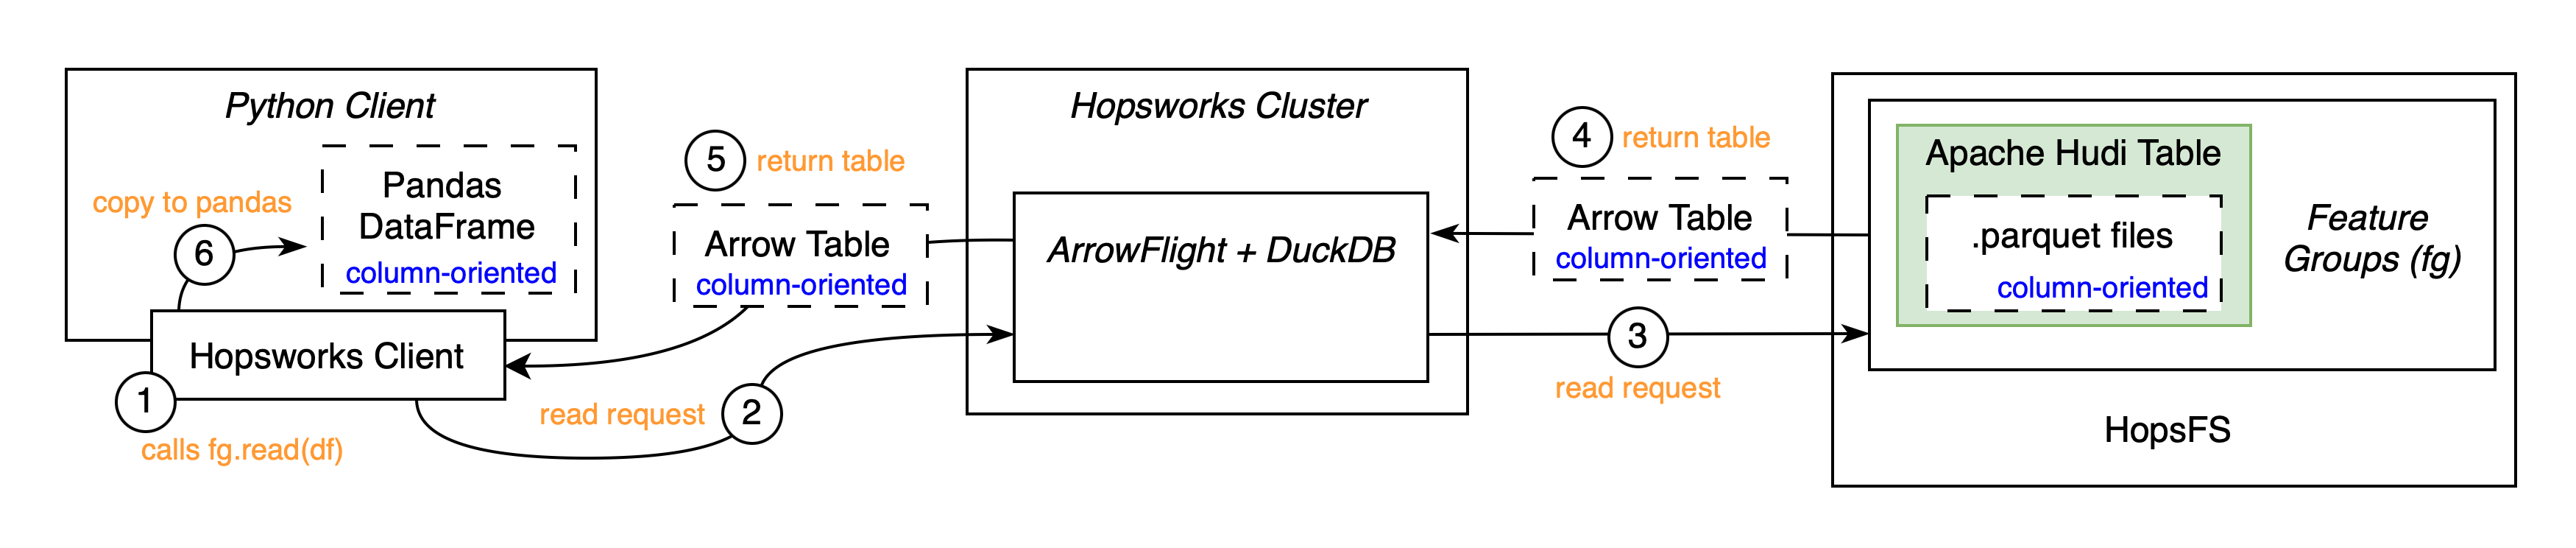
\includegraphics[width=\textwidth]{figures/2-background/FeatureStore-reading.png}
    \end{center}
    \caption[Legacy system - Read process]{Legacy system reading a table from the Hopsworks offline feature store and loading it into the Python client local memory. The process is streamlined using Arrow Tables that avoid table serialization and deserialization. Diagram inspired by the Hopsworks Feature Store paper \cite{10.1145/3626246.3653389}.}
    \label{fig:featurestore_reading}
\end{figure}

\subsection{New system - Writing}

Figure \ref{fig:delta_rs_writing} shows how the delta-rs library writes on a Delta Lake table instanced on top of \gls{HopsFS}. The delta-rs library streamlines the process, without having to pass from a server instance (Spark).

\begin{figure}
    \begin{center}
      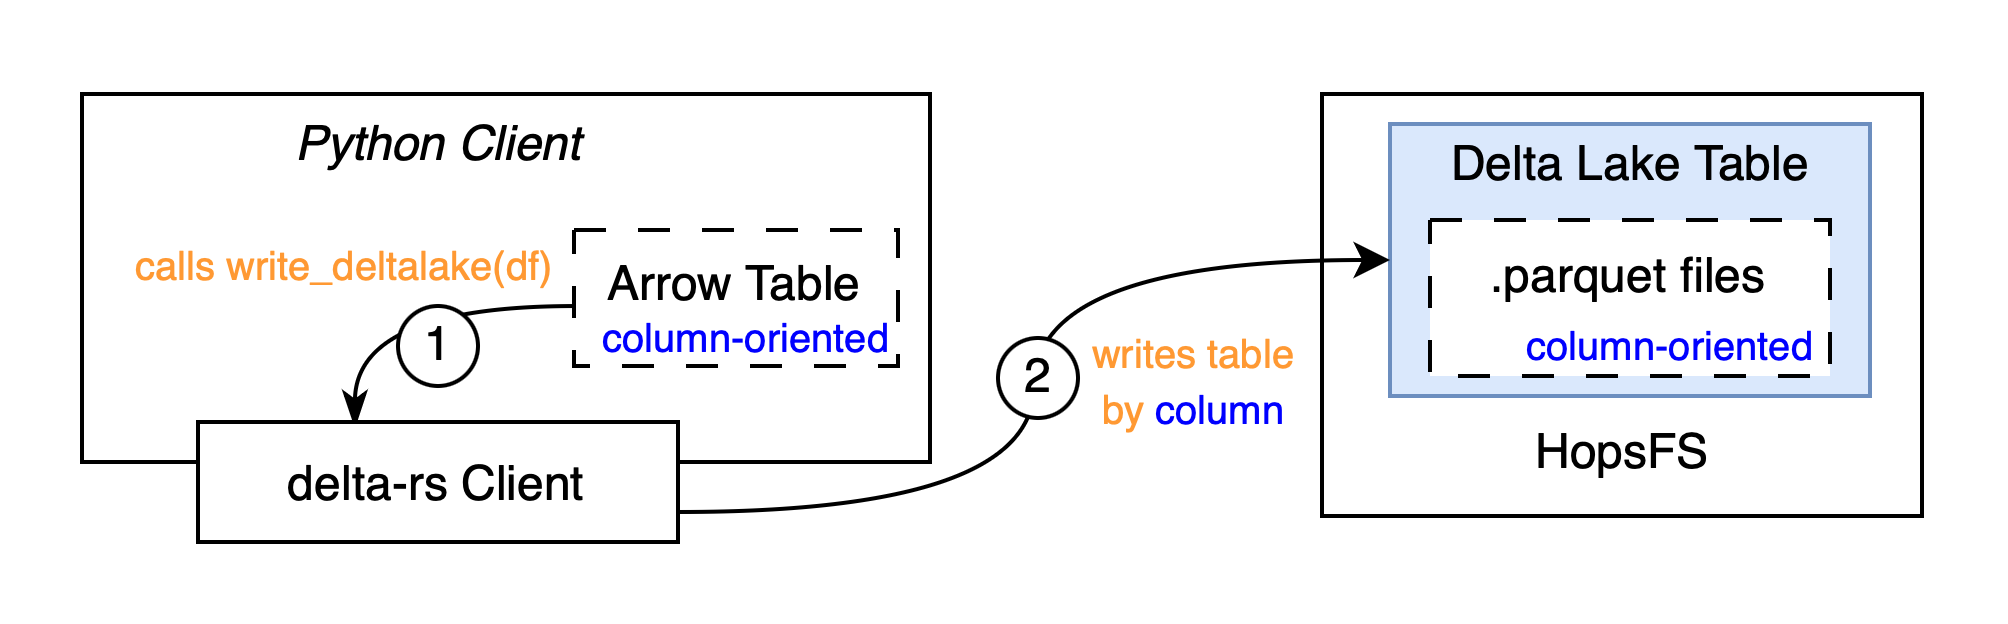
\includegraphics[width=\textwidth]{figures/2-background/delta-rs_writing.png}
    \end{center}
    \caption[Delta-rs library - Write process]{Delta-rs library writing an Arrow Table from a Python client to a Delta Lake table store on \gls{HopsFS}.}
    \label{fig:delta_rs_writing}
\end{figure}

\subsection{New system - Reading}

Figure \ref{fig:delta_rs_reading} shows how the delta-rs library reads on a Delta Lake table instanced on top of \gls{HopsFS}. The delta-rs library streamlines the process, without having to pass from a server instance (Arrow Flight).

\begin{figure}
    \begin{center}
      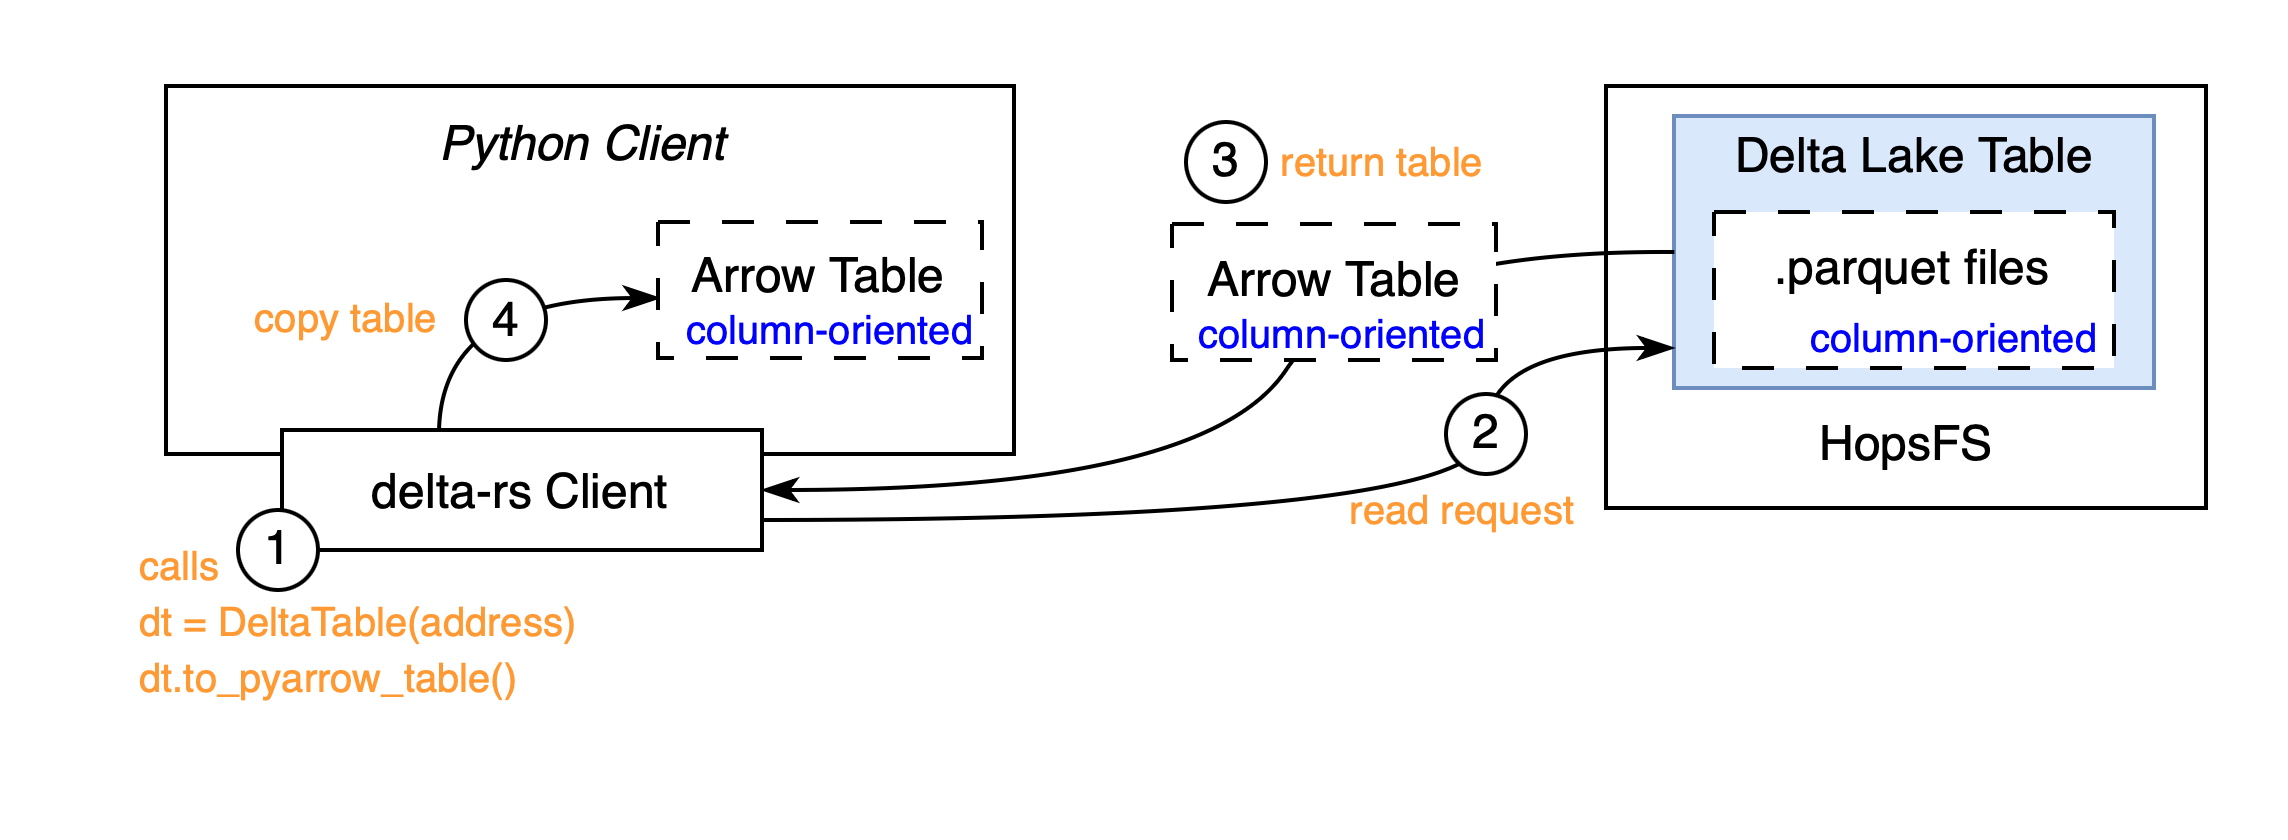
\includegraphics[width=\textwidth]{figures/2-background/delta-rs_reading.png}
    \end{center}
    \caption[Delta-rs library - Read process]{Delta-rs library reading a Delta Table stored in \gls{HopsFS} and loading it into memory.}
    \label{fig:delta_rs_reading}
\end{figure}